O objetivo desta seção é relatar as atividades desenvolvidas pelo aluno bolsista no período a que se refere este relatório. A seção \ref{sec:preproc} descreve o que foi desenvolvido na etapa de pré-processamento das imagens utilizadas (envolvendo a utilização de filtros para extração de ruído e a extração do contorno). Na seção \ref{sec:curvdisc} serão descritas as técnicas utilizadas para a análise da curvatura discreta, e a seção \ref{sec:laplacebeltrami} terá detalhes sobre a reconstrução de curvas, utilizando o método descrito em \citeonline{Sorkine2006}.

\section{Pré-processamento de imagens}\label{sec:preproc}

A primeira parte deste projeto refere-se ao pré-processamento de imagens, visando a eliminação de pontos espúrios no contorn de forma a permitir a extração de curvatura que melhor corresponda ao contorno original. A biblioteca de visão computacional \citeonline{OpenCV}, por possuir diversas funcionalidades para esta finalidade, foi utilizada neste projeto na sua versão em linguagem de programação C++.

O pré-processamento consistiu das seguintes operações:

\begin{enumerate}
% 	\item \textbf{Filtros e suavizações (Gaussiano e Perona-Malik)}. Nesta etapa foram aplicados na imagem original o filtro Gaussiano e a difusão anisotrópico de Perona-Malik, objetivando a diminuição de ruídos e suavização da imagem.
	
	\item \textbf{Filtros e suavizações (Gaussiano e Perona-Malik)}. Nesta etapa, foram testados dois tipos de suavização sobre a imagem original, aplicando o filtro Gaussiano e a difusão anisotrópica de Perona-Malik, objetivando a diminuição de ruídos e suavização da imagem. A difusão anisotrópica de Perona-Malik é mais adequada ao projeto, pois preserva as bordas da imagem \cite{hidalgo2013}, enquanto o filtro Gaussiano não \cite{szeliski2011}.
	
	\item \textbf{Conversão da imagem para tons de cinza}. Sem perda alguma de generalidade para as imagens-teste de folhas utilizadas nesta etapa, foi realizada a conversão RGB-tons de cinza, de forma a simplificar a aplicação das etapas de pré-processamento posteriores. 
	%Para facilitar a análise da imagem, os pixels (originalmente representados por uma tripla RGB, com as respectivas tonalidades de vermelho, verde e azul) tem sua cor convertida para tons de cinza, podendo assim ser representados por um inteiro de $0$ a $255$ (em que $0$ é preto e $255$ é branco).
	
	\item \textbf{Binarização por Otsu}. Teve por objetivo segmentar a imagem de folha em duas regiões: \textit{background} e \textit{foreground}. Esta segmentação é feita a partir da delimitação de um limiar, encontrado automaticamente pelo algoritmo de Otsu \cite{burger2016}.
	
	\item \textbf{Operadores morfológicos (erosão e dilatação)}. A partir da imagem binarizada, são realizadas as operações morfológicas de erosão (remoção de alguns pontos isolados e penínsulas na imagem) e a dilatação (preenchimento de alguns buracos indesejados que possam ter sido formados ou amplificados na erosão) \cite{serra1984}.
	
	\item \textbf{Extração do contorno pelo método \textit{contour-following}}. A última etapa do pré-processamento é a extração do contorno da imagem. Esta etapa consistiu da implementação do algoritmo denominado \textit{contour-following}, definido em \cite{costajr2009}, que procura o primeiro pixel pertencente ao contorno e, a partir deste, localiza, no sentido anti-horário, os próximos pixels pertencentes ao contorno, em uma vizinhança 8-conectada. Para o caso específico das imagens de folha, o contorno obtido é sempre fechado. 
	%de contorno em seus vizinhos. De acordo com a ordem que os pontos são visitados, é extraído o contorno no sentido anti-horário.
\end{enumerate}

Após o final deste fluxo de operações, obtém-se um vetor de pontos ou coordenadas $(x_i, y_i)$, referentes ao contorno do objeto segmentado. As principais etapas deste pré-processamento são ilustradas na figura \ref{img:preprocess}.

\begin{figure}[htb]
	\centering
	\caption{Resultados da etapa de pré-processamento.}
	\begin{subfigure}[t]{0.24\textwidth}
		\centering
		\includegraphics[width=1\textwidth]{img/original.jpg}
		\caption{Folha original}
	\end{subfigure}
	\begin{subfigure}[t]{0.24\textwidth}
		\centering
		\includegraphics[width=1\textwidth]{img/perona.jpg}
		\caption{Após suavização por Perona-Malik}
	\end{subfigure}
	\begin{subfigure}[t]{0.24\textwidth}
		\centering
		\includegraphics[width=1\textwidth]{img/preprocess.jpg}
		\caption{Após segmentação por Otsu}
	\end{subfigure}
	\begin{subfigure}[t]{0.24\textwidth}
		\centering
		\includegraphics[width=1\textwidth]{img/contour.jpg}
		\caption{Contorno extraído}
	\end{subfigure}
	\legend{Fonte: original de \citeonline{imageclef2011}, e edições elaboradas pelo autor.}
	\label{img:preprocess}
\end{figure}

\section{Análise da curvatura}\label{sec:curvdisc}

A análise de curvatura é importante para a possibilitar a posterior extração de dos pontos importantes. A curvatura de uma curva regular parametrizada por uma aplicação $t \rightarrow (x(t), y(t))$, onde $x(t)$ e $y(t)$ são funções de classe $C^2$, é dada por \cite{OliveiraMarroquim2020}:

\begin{equation}
    \kappa (t) = \frac{x'(t) y''(t) - y'(t) x''(t)}{(x'(t)^2 + y'(t)^2)^{3/2}}.
\end{equation}

Porém, no escopo do projeto, como a curva é representada por um conjunto discreto de pontos $(x, y)$ - que representam a posição de cada pixel - as derivadas devem ser calculadas de forma discreta. Este cálculo pode ser realizado a partir de métodos espectrais de Fourier \cite{brethwashington}.

Seja $u_j$ uma aproximação discreta da função $u(x)$, com $n$ pontos de amostra $x_j \in h, 2h, \dots, ih, \dots, 2\pi - h, 2\pi$, onde $h = 2\pi/n$. Para o caso discreto, pode-se aplicar a versão computacionalmente otimizada da transformada de Fourier (FFT) em $u_j$, tal que $FFT(u_j) \equiv \hat{u}_k$, em que $k \in \frac{-n}{2}+1, \dots, \frac{n}{2}$. Sabe-se que:

$$FFT \left (\frac{\partial u_j}{\partial x} \right) \equiv i k \hat{u}_k$$

Assim, para obter o valor da derivada, basta calcular a transformada rápida inversa IFFT. O código MATLAB apresentado abaixo calcula a derivada de uma função discreta $y$ no domínio $x$ e emprega um filtro Gaussiano com fator de suavização $\sigma$. A aplicação de um filtro Gaussiano no cálculo da derivada tem por objetivo evitar a amplificação do efeito de serrilhamento (\textit{aliasing}), quando houver, causado pela transformada de Fourier \cite{li1987}. O filtro Gaussiano cumpre este objetivo ao eliminar altas frequências presentes no sinal com a propriedade de preservar a localização de pontos importantes da mudança da curvatura \cite{tomasi2007}.
%Para amenizar possíveis ruídos que ainda existam, pode-se também utilizar um filtro Gaussiano. A seguir, uma função em MATLAB que calcula a derivada de uma função discreta $y$ no domínio $x$, utilizando um determinado $\sigma$ para a suavização Gaussiana:

\noindent\rule{0.95 \textwidth}{1.pt}
\vspace{-0.2cm}
\begin{verbatim}
function [ dy ] = calcDerivative(sigma, y, x)
  % calcDerivative Calcula a derivada de uma funcao y(x) discreta
  
  n = size(x, 2); % qtt de pontos
  st = 1.0 / (x(1, n) - x(1, 1)); % step para x_i
  X = (-floor(n/2):(n - floor(n/2) - 1)) * st; % shift do domínio
  GAU = exp(-((X.^2)/(sigma^2))/2); % filtro gaussiano
  GAU = fftshift(GAU);

  % fft e aplicacao do filtro gaussiano
  y = fft(fftshift(y));
  A = (GAU .* y);

  % funcao derivada
  DER = 2*pi*1i*X;
  DER = fftshift(DER);
  dy = ifftshift(real(ifft(A .* DER)));
end
\end{verbatim}
\vspace{-0.5cm}
\noindent\rule{0.95 \textwidth}{1.pt}\\

Um exemplo do cálculo da curvatura pode ser visto na figura \ref{img:curv}. Nela, foi utilizado o contorno da imagem ilustrada na figura \ref{img:preprocess}. Para facilitar a visualização do gráfico, o ponto destacado em preto é o ponto inicial da curvatura, e os demais pontos seguem sentido horário.

\begin{figure}[htb]
	\centering
	\caption{Curvatura calculada para o contorno.}
	\begin{subfigure}[b]{0.22\textwidth}
		\centering
		\includegraphics[trim={2cm 1cm 0 0},clip,width=1\textwidth]{img/contorno.jpg}
		\caption{Contorno original}
	\end{subfigure}
	\begin{subfigure}[b]{0.73\textwidth}
		\centering
		\includegraphics[width=1\textwidth]{img/curvatura.jpg}
		\caption{Curvatura calculada}
	\end{subfigure}
	\legend{Fonte: Elaborada pelo autor.}
	\label{img:curv}
\end{figure}

\section{Reconstrução de curvas}\label{sec:laplacebeltrami}

Nesta seção serão abordadas as atividades realizadas sobre a reconstrução de curvas a partir de poucos pontos e de informações de conectividade. Para isso, foram utilizadas coordenadas diferenciais, como descrito em \citeonline{Sorkine2006}.

Seja $\mathcal{M} = (V, E, F)$ uma malha triangular caracterizada, respectivamente, por seus conjuntos de vértices, arestas e faces, e cada vértice $\mathbf{v}_i \in V$ possui uma coordenada cartesiana dada por $\mathbf{v}_i = (x_i,y_i,z_i)$. As coordenadas diferenciais (ou $\delta$-coordenadas) são definidas como:

\begin{equation}
	\mathbf{\delta}_i = (\mathbf{\delta}_i^{(x)}, \mathbf{\delta}_i^{(y)}, \mathbf{\delta}_i^{(z)}) = \mathbf{v}_i - \frac{1}{d_i} \sum_{j \in N(i)} \mathbf{v}_j,
	\label{eq_delta}
\end{equation}

\noindent em que $N(i) = \{j\ |\ (i,j) \in E$\} (ou seja, o conjunto dos vértices adjacentes a $i$) e $d_i = |N(i)|$ é o número dos vizinhos imediatos de $i$ (grau de $i$).

Caso a malha $\mathcal{M}$ seja uma aproximação de superfície linear por partes, a coordenada diferencial $\delta_i$ pode ser vista como a discretização da seguinte integral:

\begin{equation}
	\frac{1}{|\gamma|} \int_{\mathbf{v} \in \gamma} (\mathbf{v}_i - v) dl(\mathbf{v}))
\end{equation}

\noindent onde $\gamma$ é uma superfície simples e fechada em torno de $\mathbf{v}$ e $|\gamma|$ é o comprimento de $\gamma$. Sabe-se, de geometria diferencial \cite{manfredo2014}, que

\begin{equation}
	\lim_{|\gamma| \rightarrow 0} \frac{1}{|\gamma|} \int_{\mathbf{v} \in \gamma} (\mathbf{v}_i - \mathbf{v}) dl(\mathbf{v}) = -H(\mathbf{v}_i)\mathbf{n}_i
\end{equation}

\noindent em que $H(\mathbf{v}_i)$ é a curvatura média em $\mathbf{v}_i$ e $\mathbf{n}_i$ é o vetor normal à superfície. Assim, as $\mathbf{\delta}$-coordenadas podem ser vistas como a discretização do operador contínuo de Laplace-Beltrami, e a direção do vetor de coordenadas diferenciais aproxima-se à direção normal e sua norma aproxima a quantidade proporcional à curvatura média local. De maneira resumida, isto significa que as $\mathbf{\delta}$-coordenadas encapsulam a forma da superfície local.

A transformação das coordenadas cartesianas absolutas para as $\delta$-coordenadas também pode ser calculada em forma de matriz. Seja $A$ a matriz de adjacências da malha e $D$ matriz diagonal tal que $D_{ii} = d_i$ (grau do vértice $i$), a matriz transformação de coordenadas absolutas para as diferenciais é:

\begin{equation}
	L = I - D^{-1}A.
\end{equation}

Porém, é mais conveniente (e computacionalmente eficiente) utilizar a versão simétrica $L_s$ da matriz $L$, definida por:

\begin{equation}\label{eqMatLaplaciana}
	L_s = DL = D - A
\end{equation}

\noindent em que cada célula pode ser calculada da seguinte forma:

\begin{equation}
	(L_s)_{ij} = \begin{cases}
		d_i&i=j\\
		-1&(i, j) \in E\\
		0&\text{caso contrário.}
	\end{cases}
\end{equation}

Esta matriz $L_s$ é denominada \textit{Laplaciano topológico} da malha $\mathcal M$. Um exemplo dela pode ser visto na figura \ref{fig:grafo_lapl}.

\begin{figure}[htb]
    \centering
    \caption{Malha bidimensional e seu laplaciano topológico}
    \includegraphics{img/grafo_lapl.png}
    \legend{Fonte: Elaborada pelo autor.}
    \label{fig:grafo_lapl}
\end{figure}

Porém, a conversão das $\delta$-coordenadas de volta para as cartesianas exige mais atenção. As coordenadas diferenciais são invariantes à translação, pois caso a malha $\mathcal{M}$ seja transladada de acordo com um vetor $u$ gerando novos vértices $v_i'$, tem-se:

\begin{align*}
	L(\mathbf{v}_i') &= \sum_{j \in N(i)} w_{ij} (\mathbf{v}_i' - \mathbf{v}_j')\\ 
	&= \sum_{j \in N(i)} w_{ij} ((\mathbf{v}_i + \mathbf{u})  - (\mathbf{v}_j + \mathbf{u}))\\ 
	&= \sum_{j \in N(i)} w_{ij} (\mathbf{v}_i - \mathbf{v}_j) = L(\mathbf{v}_i)
\end{align*}

Assim, as matrizes $L$ e $L_s$ são singulares, e $\mathbf{x} = L_s^{-1} \mathbf{\delta}^{(x)}$ é indefinido. Mais que isso, como cada componente da malha possui um grau de liberdade de translação, tem-se que $rank(L) = n - k$, em que $k$ é o número de componentes. Para que seja possível restaurar as coordenadas absolutas, é necessário que o sistema linear seja \textit{full-rank} - e isto pode ser alcançado adicionando restrições para fixar a localização de alguns vértices, denominados pontos âncora. Suponha que sejam fixados a localização de $m$ vértices com índices $P = \{1, 2, \cdots, m\}$, em que são conhecidas as localizações $c = \{\mathbf{v}_j\ |\ j \in P\}$. Serão adicionadas restrições do tipo:

$$\mathbf{v}_j = \mathbf{c_j}, \forall\ j \in P$$

Com a denotação matricial, o novo sistema linear será:

\begin{equation}\label{eq:sisrecover}
	\left( \frac{L}{\omega I_{m \times m} | 0} \right) \mathbf{x} = \begin{pmatrix}
		\delta^{(x)}\\
		\omega\ c_{1:m}^{(x)}
	\end{pmatrix}
\end{equation}

\noindent e o mesmo vale para os outros vetores de coordenadas. Com a utilização do vetor $\omega > 0$, cada restrição pode possuir um peso diferente, que pode ajustar a importância e relevância de cada vértice.

Graficamente, pode-se representar o sistema da seguinte maneira: 

\begin{center}
	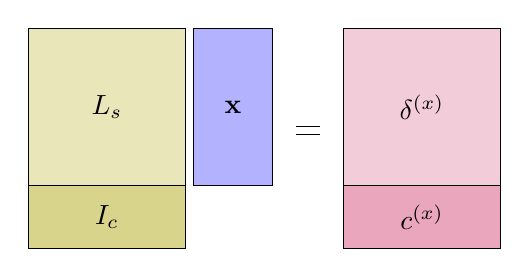
\begin{tikzpicture}
		\filldraw[fill=olive!20!white, draw=black] (0,0) rectangle node{$L_s$} (2,2);
		\filldraw[fill=olive!35!white, draw=black] (0,0) rectangle node{$I_c$} (2,-0.8);
		\filldraw[fill=blue!30!white, draw=black] (2.1,0) rectangle node{$\mathbf{x}$} (3.1,2);
		\draw (3.4, 0.65) -- (3.7, 0.65);
		\draw (3.4, 0.75) -- (3.7, 0.75);
		\filldraw[fill=purple!20!white, draw=black] (4,0) rectangle node{$\delta^{(x)}$} (6,2);
		\filldraw[fill=purple!35!white, draw=black] (4,0) rectangle node{$c^{(x)}$} (6,-0.8);
	\end{tikzpicture}
\end{center}

\noindent onde, $I_c$ é a matriz identidade $m \times m$, com zeros à direita (e foi fixado $\omega = 1$ por simplicidade).

A matriz dos coeficientes em \ref{eq:sisrecover} é denominada $\tilde{L}$. Por mais que o sistema tenha mais equações que incógnitas, ele é \textit{full-rank} e possui uma única solução com a utilização do método dos mínimos quadrados:

\begin{equation}\label{eq:leastsqrsol}
	\mathbf{\tilde{x}} = \mathop{\mathrm{argmin}}_x \left( \lVert L \mathbf{x} - \delta^{(x)} \rVert^2 + \sum_{j \in C} \omega^2 \lvert x_j - c_j \rvert^2  \right)
\end{equation}

Um exemplo de fixação de pontos âncora e a respectiva matriz $\tilde{L}$ é dado na figura \ref{fig:grafo_lapl_tilde}.

\begin{figure}[htb]
    \centering
    \caption{Pontos âncora destacados em azul e seu referente $\tilde{L}$}
    \includegraphics{img/grafo_lapl_tilde.png}
    \legend{Fonte: Elaborada pelo autor.}
    \label{fig:grafo_lapl_tilde}
\end{figure}

Algumas aplicações interessantes são possíveis a partir do mapeamento entre coordenadas absolutas e diferenciais, como representação eficiente de formas, edição e interpolação de malhas. Neste projeto, com o objetivo de reconstrução das curvas, as coordenadas diferenciais serão utilizadas por representarem formas de maneira eficiente.

Se utilizada uma boa base para representação, é necessária apenas uma parcela da função de base para representar toda a geometria \cite{sorkine2004}. Desta forma, com apenas informações de conectividade da malha e alguns pontos fixados (denominados vértices âncora), é possível aproximar toda a geometria, a partir da resolução do sistema pelo método dos mínimos quadrados:

\begin{equation}\label{eq:sisrecover2}
	\left( \frac{L}{\omega I_{m \times m} | 0} \right) \mathbf{x'} = \begin{pmatrix}
		0\\
		\omega\ c_{1:m}^{(x)}
	\end{pmatrix}
\end{equation}

\noindent em que $c = \{v_1, v_2, \dots, v_m\}$ são os pontos âncora escolhidos como amostra, e $\omega > 0$ é o peso de cada restrição. Ou seja, o sistema a ser resolvido é o mesmo da equação \ref{eq:sisrecover}, porém o $\delta$ é substituído por $0$.

Análoga à representação gráfica apresentada anteriormente, pode-se representar o sistema da seguinte maneira:

\begin{center}
	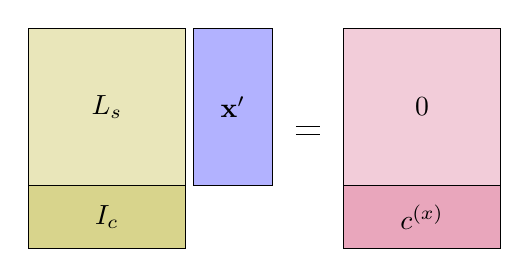
\begin{tikzpicture}
		\filldraw[fill=olive!20!white, draw=black] (0,0) rectangle node{$L_s$} (2,2);
		\filldraw[fill=olive!35!white, draw=black] (0,0) rectangle node{$I_c$} (2,-0.8);
		\filldraw[fill=blue!30!white, draw=black] (2.1,0) rectangle node{$\mathbf{x}'$} (3.1,2);
		\draw (3.4, 0.65) -- (3.7, 0.65);
		\draw (3.4, 0.75) -- (3.7, 0.75);
		\filldraw[fill=purple!20!white, draw=black] (4,0) rectangle node{$0$} (6,2);
		\filldraw[fill=purple!35!white, draw=black] (4,0) rectangle node{$c^{(x)}$} (6,-0.8);
	\end{tikzpicture}
\end{center}


É possível visualizar resultados desta reconstrução nas figuras \ref{fig:ex1rep} e \ref{fig:ex2rep}. No caso, os pontos âncoras foram escolhidos utilizando-se alguns pontos igualmente espaçados em quantidades arbitrárias. Porém, no escopo do projeto, isto será posteriormente realizado de uma maneira mais inteligente, com pontos escolhidos por informações de curvatura. Nas figuras, os pontos destacados são os pontos âncora, a curva original está em vermelho e a curva reconstruída em azul. O erro de cada reconstrução (presente na legenda de cada respectiva figura) é calculado pela soma dos erros de cada ponto, que por si são calculados como a distância Euclidiana entre os pontos recuperados e os pontos originais. Ou seja, para cada índice de vértice $i$, o erro dos pontos obtidos $\mathbf{v'}$ em relação aos pontos originais $\mathbf{v}$ é:

$$E_i(\mathbf{v, v'}) = \sqrt{(\mathbf v_i^{(x)} - \mathbf v_i'^{(x)})^2 + (\mathbf v_i^{(y)} - \mathbf v_i'^{(y)})^2}$$

\noindent e o erro total da reconstrução é calculado como:

$$E(\mathbf{v, v'}) = \sum_{i = 1}^{|V|}E_i(\mathbf{v, v'})$$

\begin{figure}[ht!]
	\centering
	\caption{Representação da função paramétrica $(x(t), y(t)) = (sin(t) + 0.5 sen(2t), -cos(t) - 0.5 - 0.5 cos(2t))$ utilizando alguns pontos igualmente espaçados como amostra.}
	\begin{subfigure}[b]{0.31\textwidth}
		\centering
		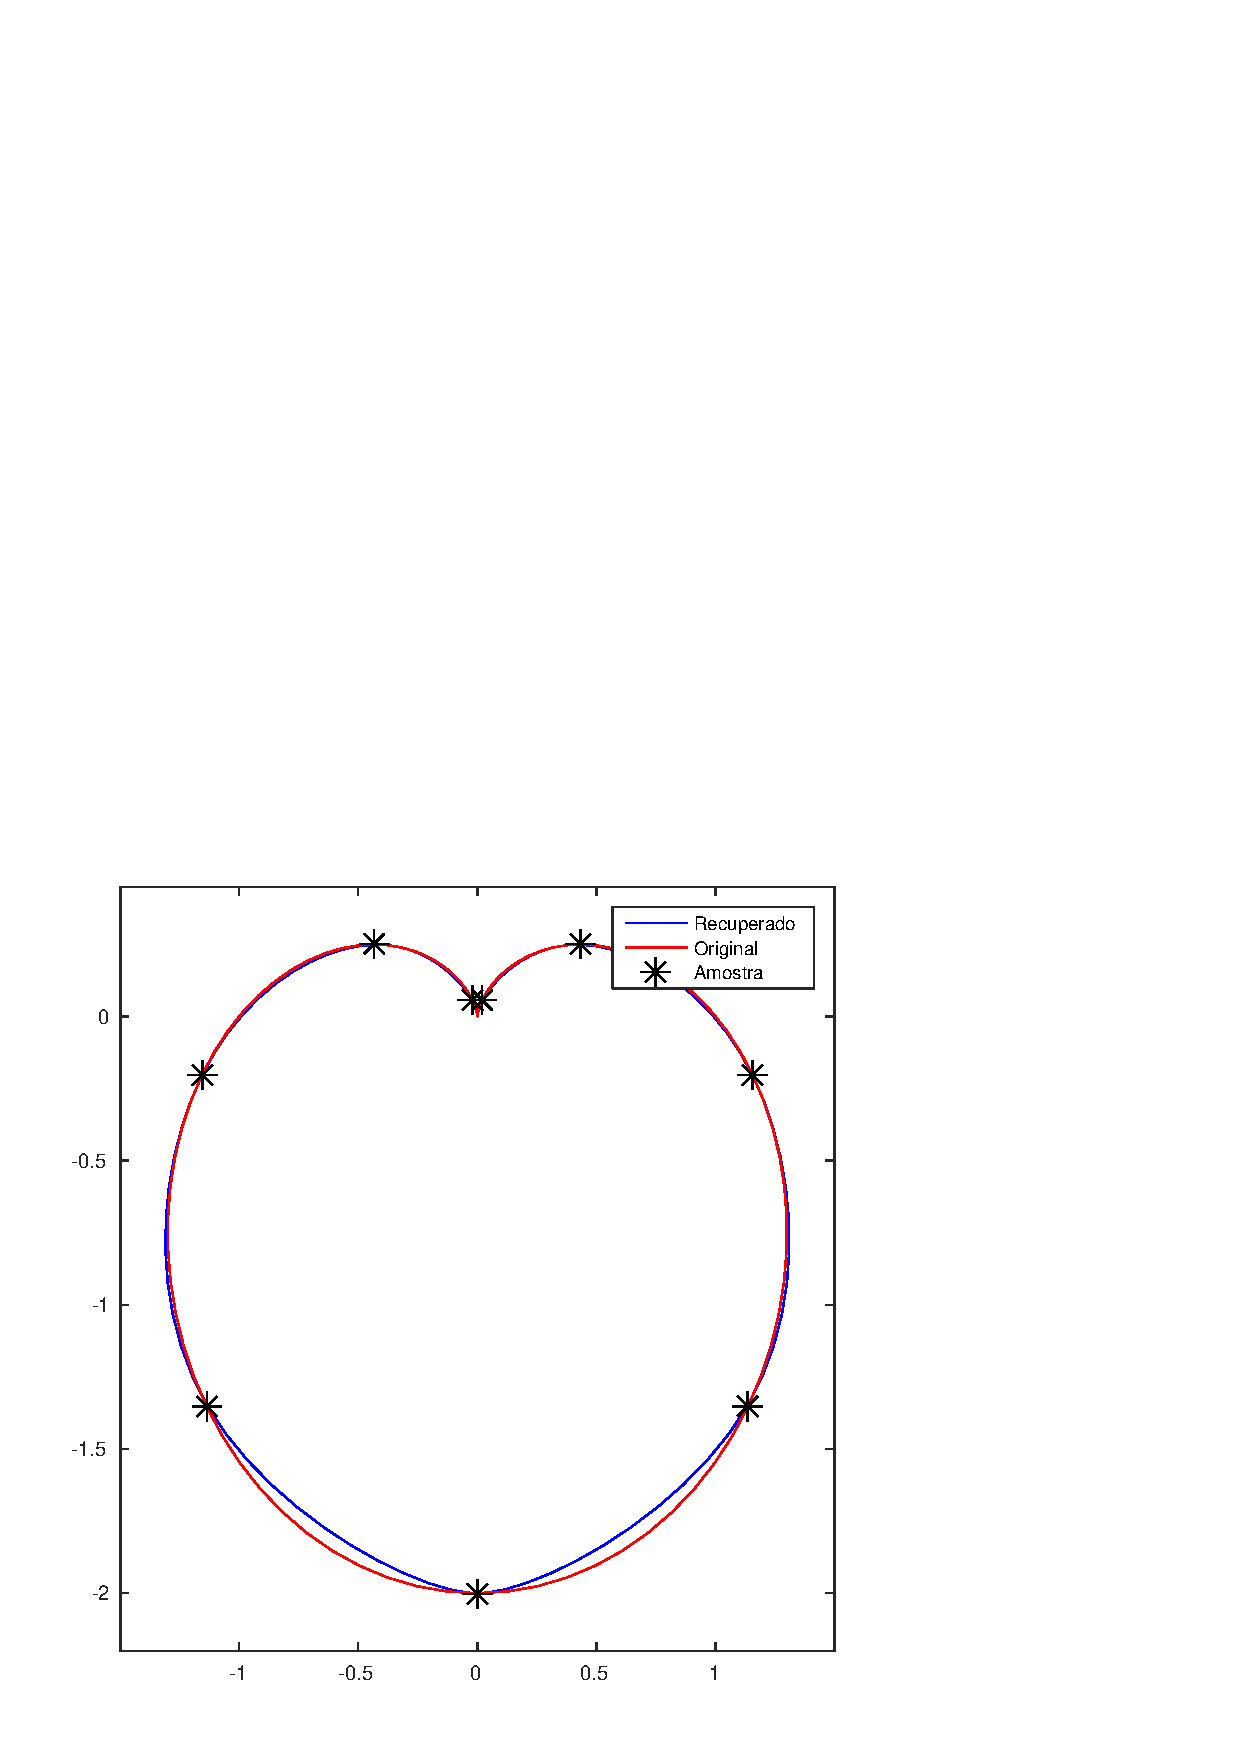
\includegraphics[trim={5cm 2cm 3cm 2cm},clip,width=\textwidth]{img/rep_1_10.jpg}
		\caption{10 pontos. Erro = 3.7199}
		\label{fig:ex14}
	\end{subfigure}
	\hfill
	\begin{subfigure}[b]{0.31\textwidth}
		\centering
		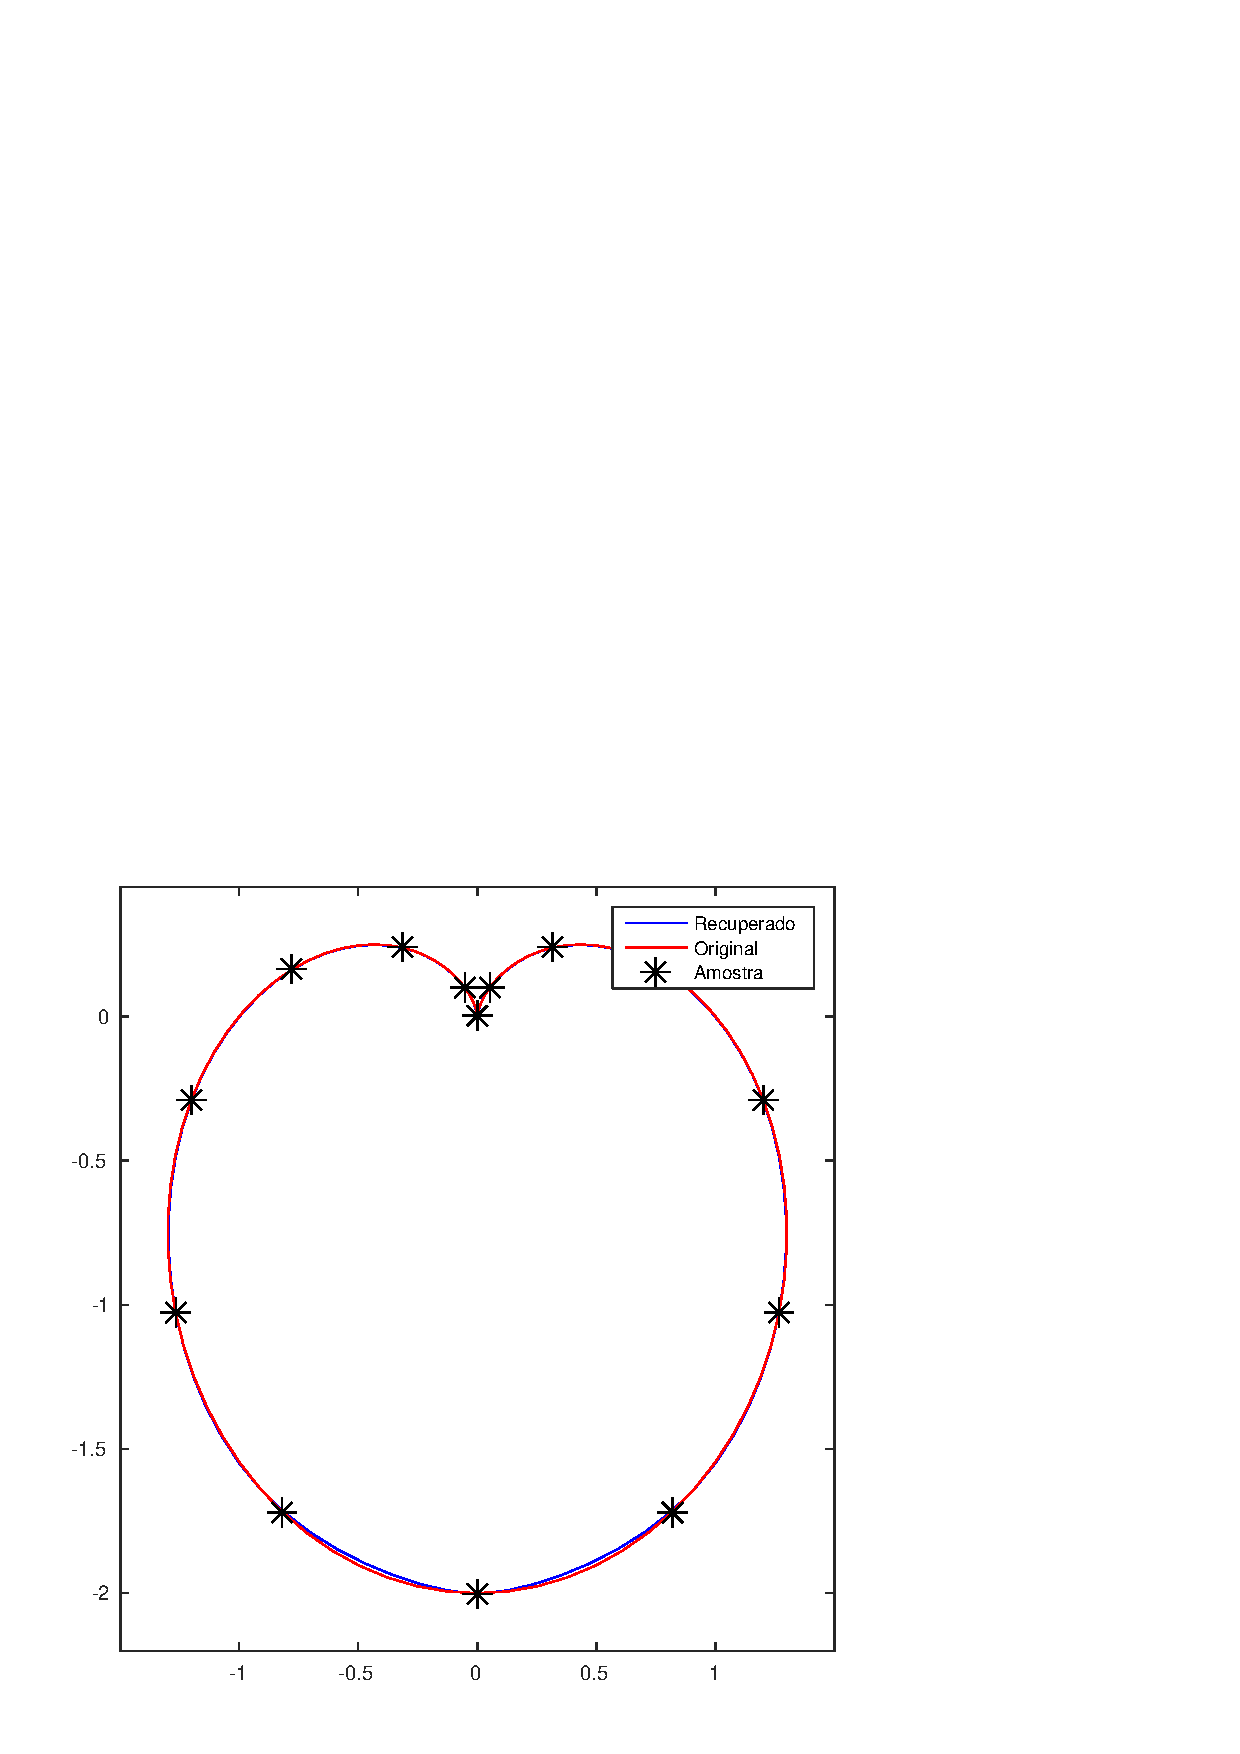
\includegraphics[trim={5cm 2cm 3cm 2cm},clip,width=\textwidth]{img/rep_1_15.jpg}
		\caption{15 pontos. Erro = 0.4498}
		\label{fig:ex12}
	\end{subfigure}
	\hfill
	\begin{subfigure}[b]{0.31\textwidth}
		\centering
		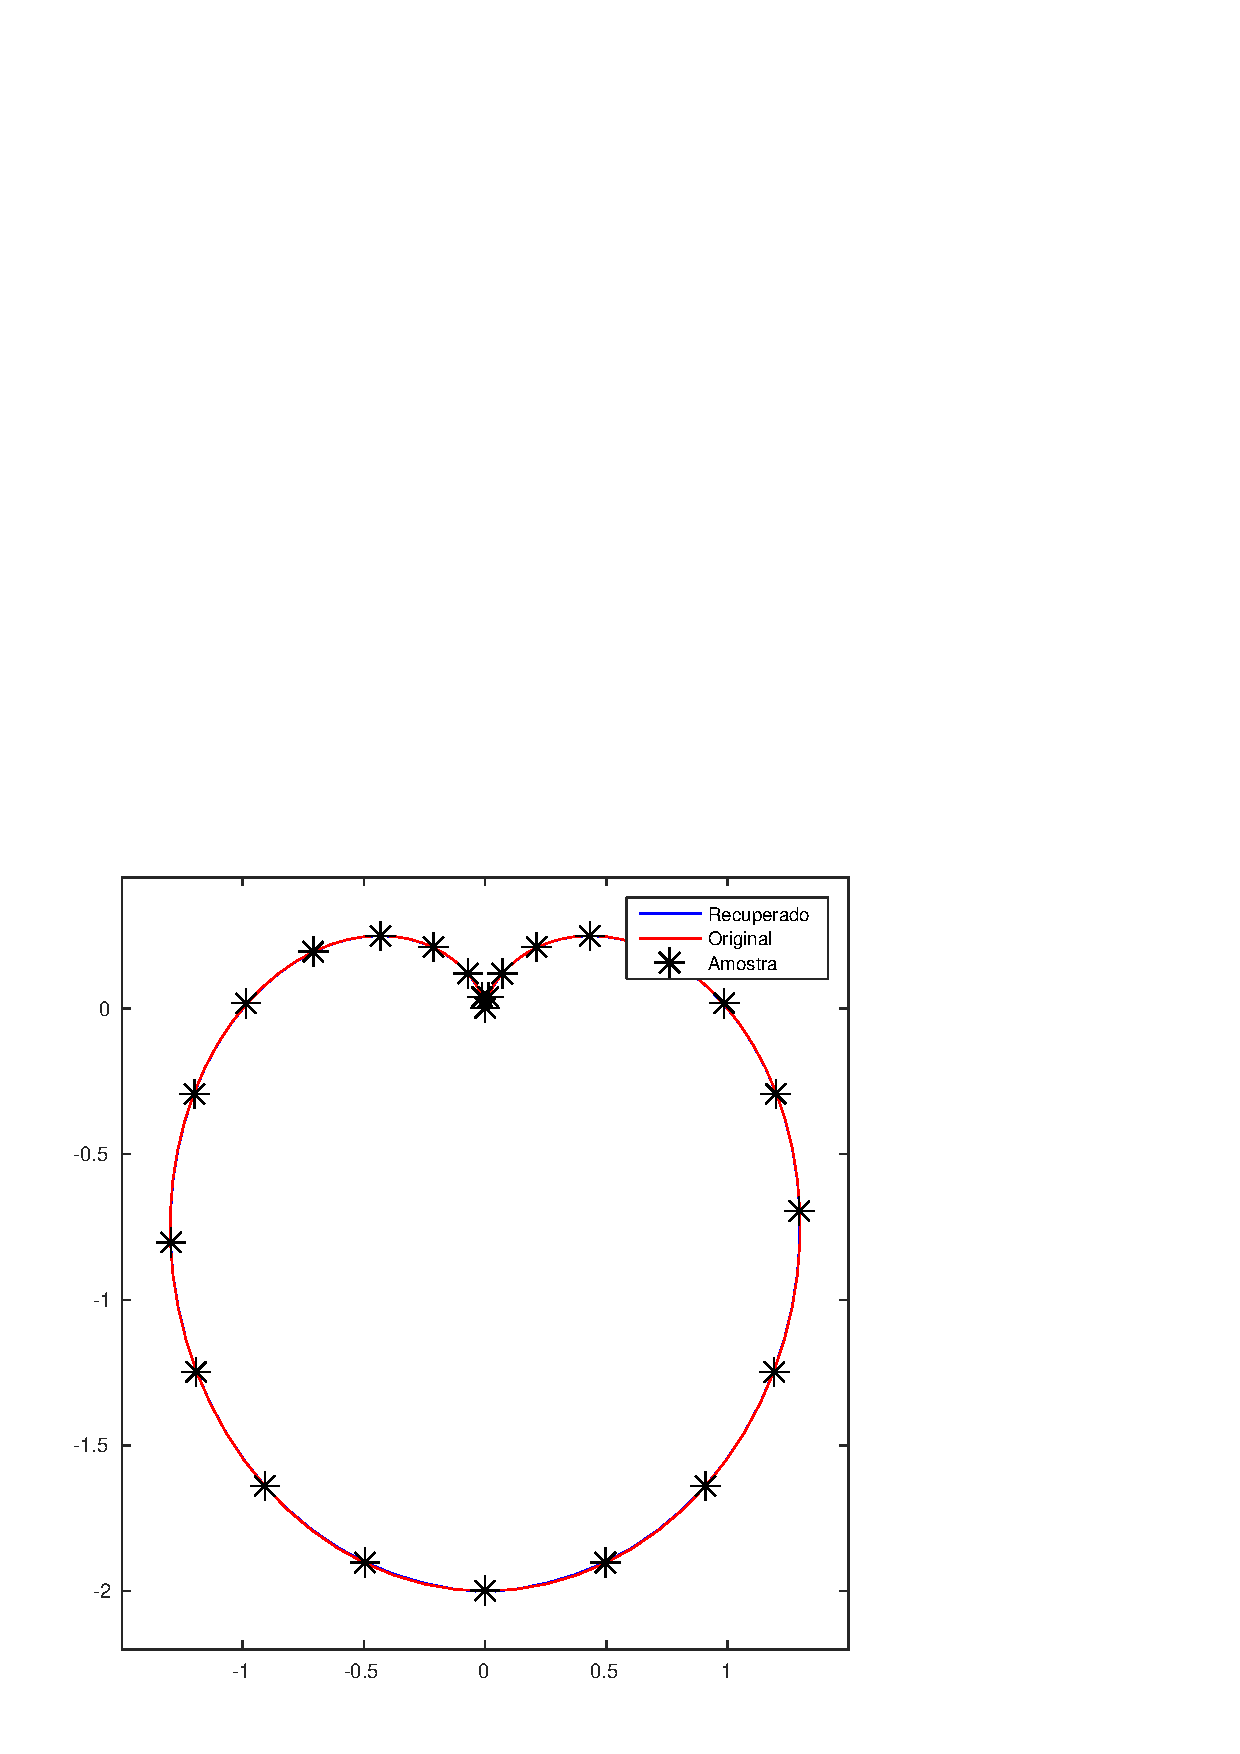
\includegraphics[trim={5cm 2cm 3cm 2cm},clip,width=\textwidth]{img/rep_1_25.jpg}
		\caption{25 pontos. Erro = 0.2045}
		\label{fig:ex13}
	\end{subfigure}
	\legend{Fonte: Elaborada pelo autor.}
	\label{fig:ex1rep}
\end{figure}

\begin{figure}[ht!]
	\centering
	\caption{Representação da função paramétrica $(x(t), y(t)) = (3 cos(3t), 5sen(2t))$ utilizando alguns pontos igualmente espaçados como amostra.}
	\begin{subfigure}[b]{0.31\textwidth}
		\centering
		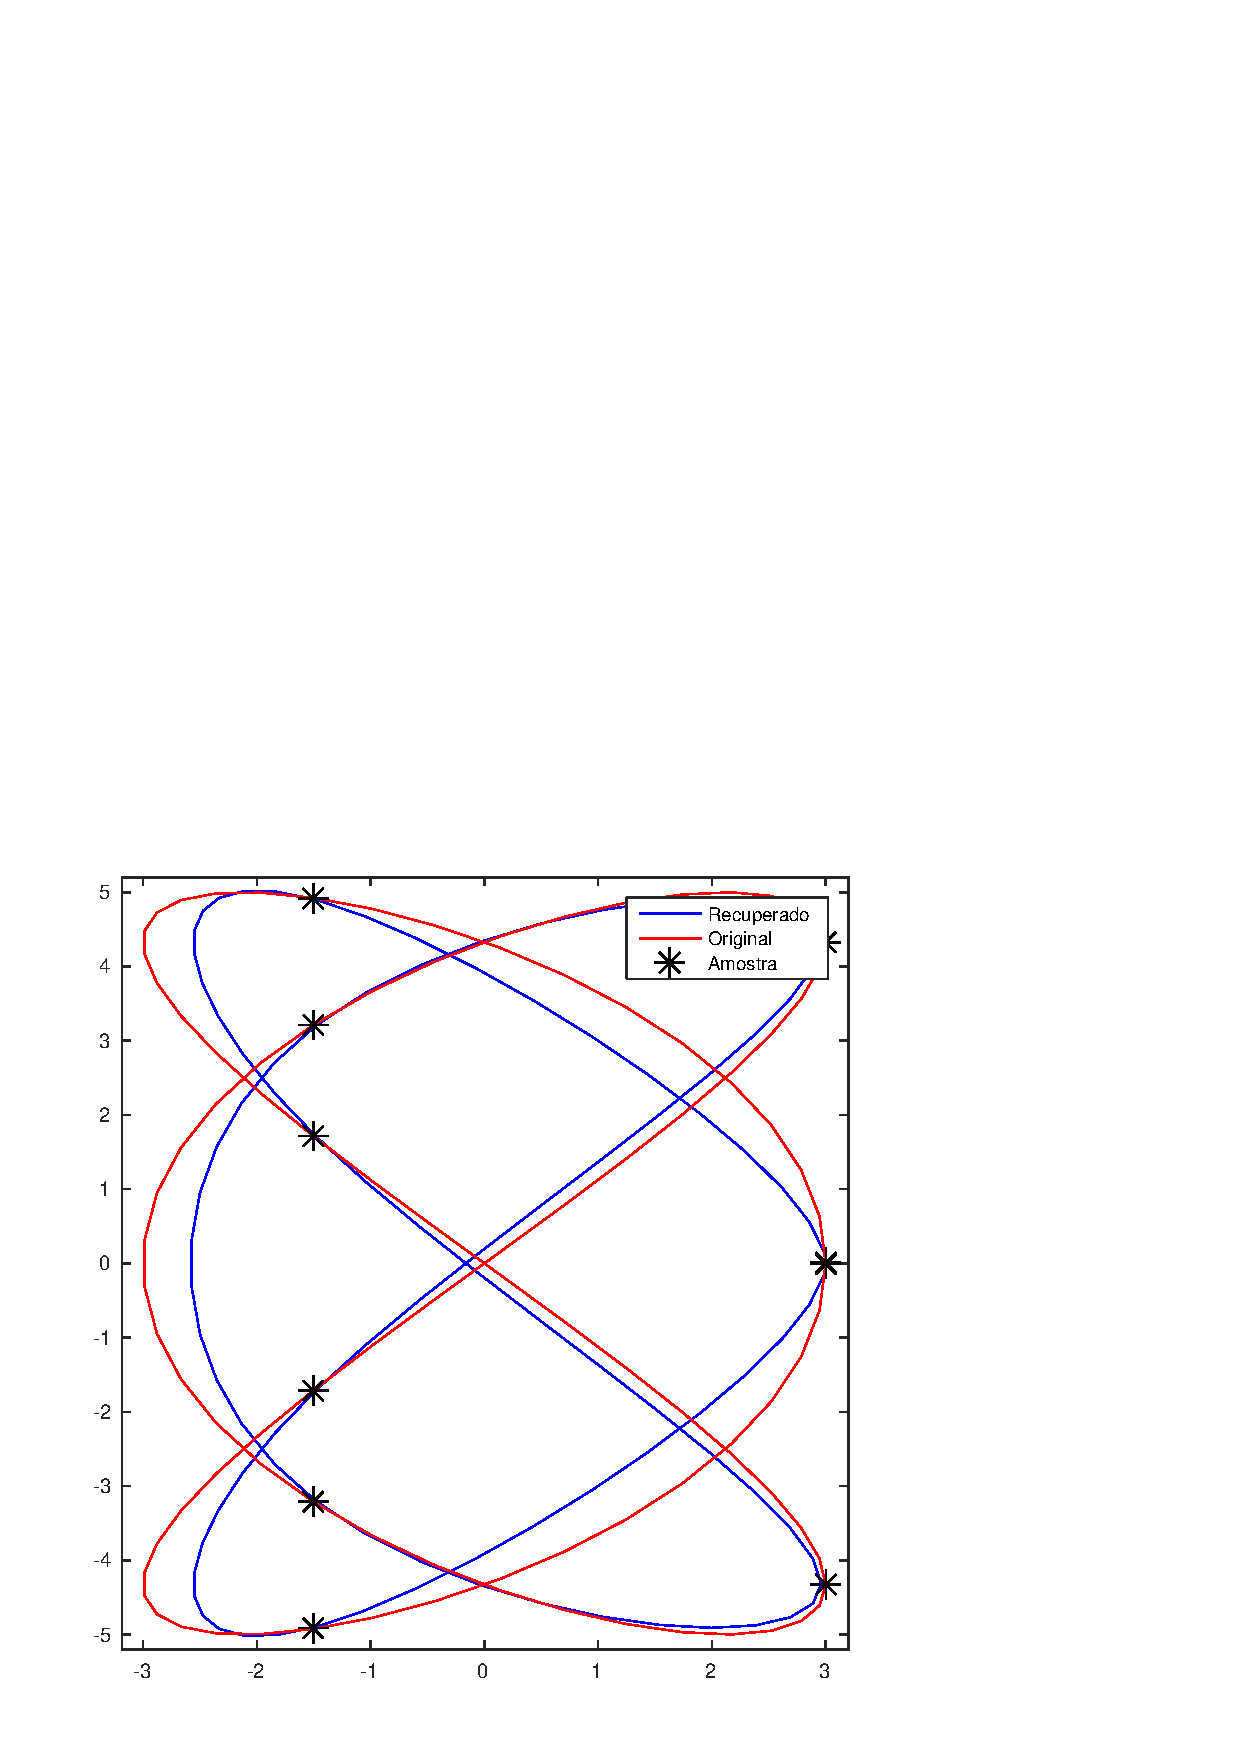
\includegraphics[trim={5cm 2cm 3cm 2cm},clip,width=\textwidth]{img/rep_2_10.jpg}
		\caption{10 pontos. Erro = 75.2102}
		\label{fig:ex24}
	\end{subfigure}
	\hfill
	\begin{subfigure}[b]{0.31\textwidth}
		\centering
		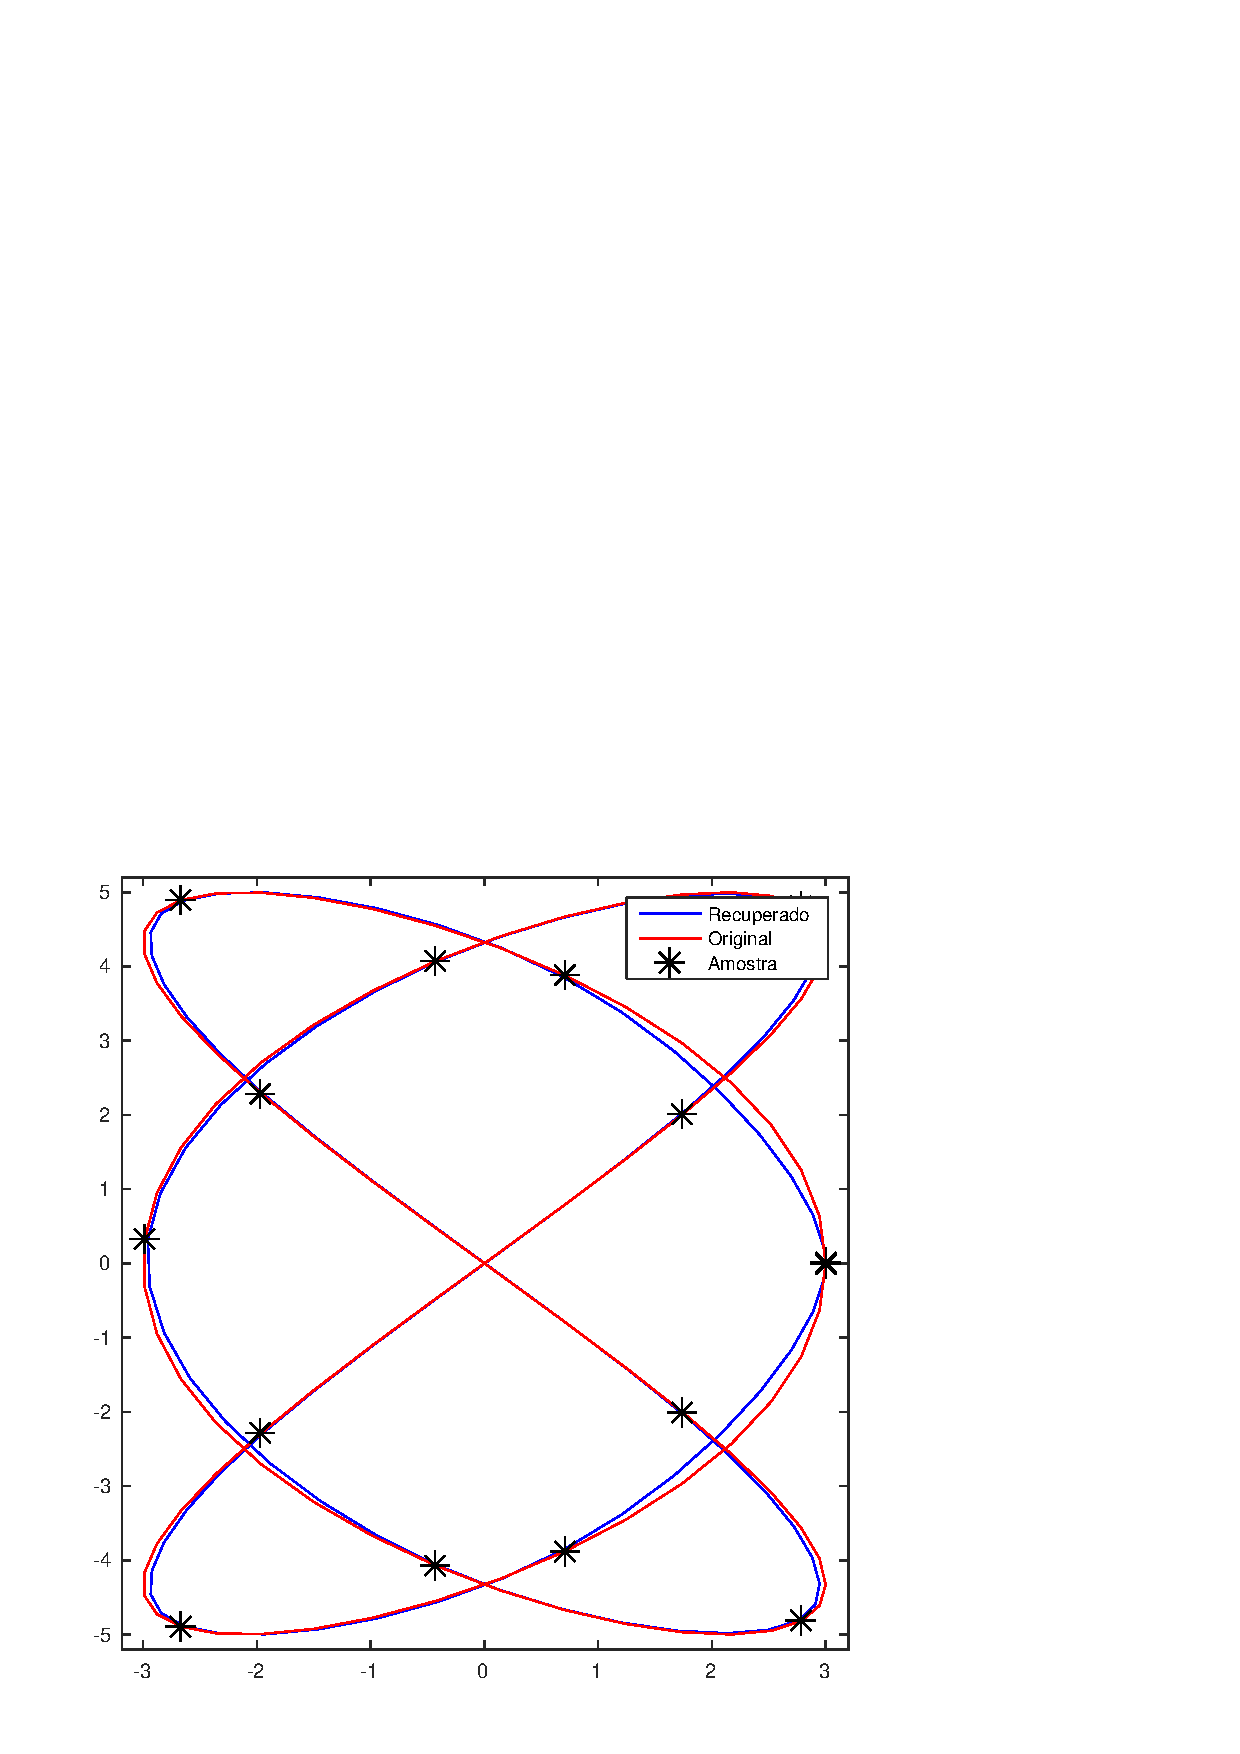
\includegraphics[trim={5cm 2cm 3cm 2cm},clip,width=\textwidth]{img/rep_2_15.jpg}
		\caption{15 pontos. Erro = 4.8213}
		\label{fig:ex22}
	\end{subfigure}
	\hfill
	\begin{subfigure}[b]{0.31\textwidth}
		\centering
		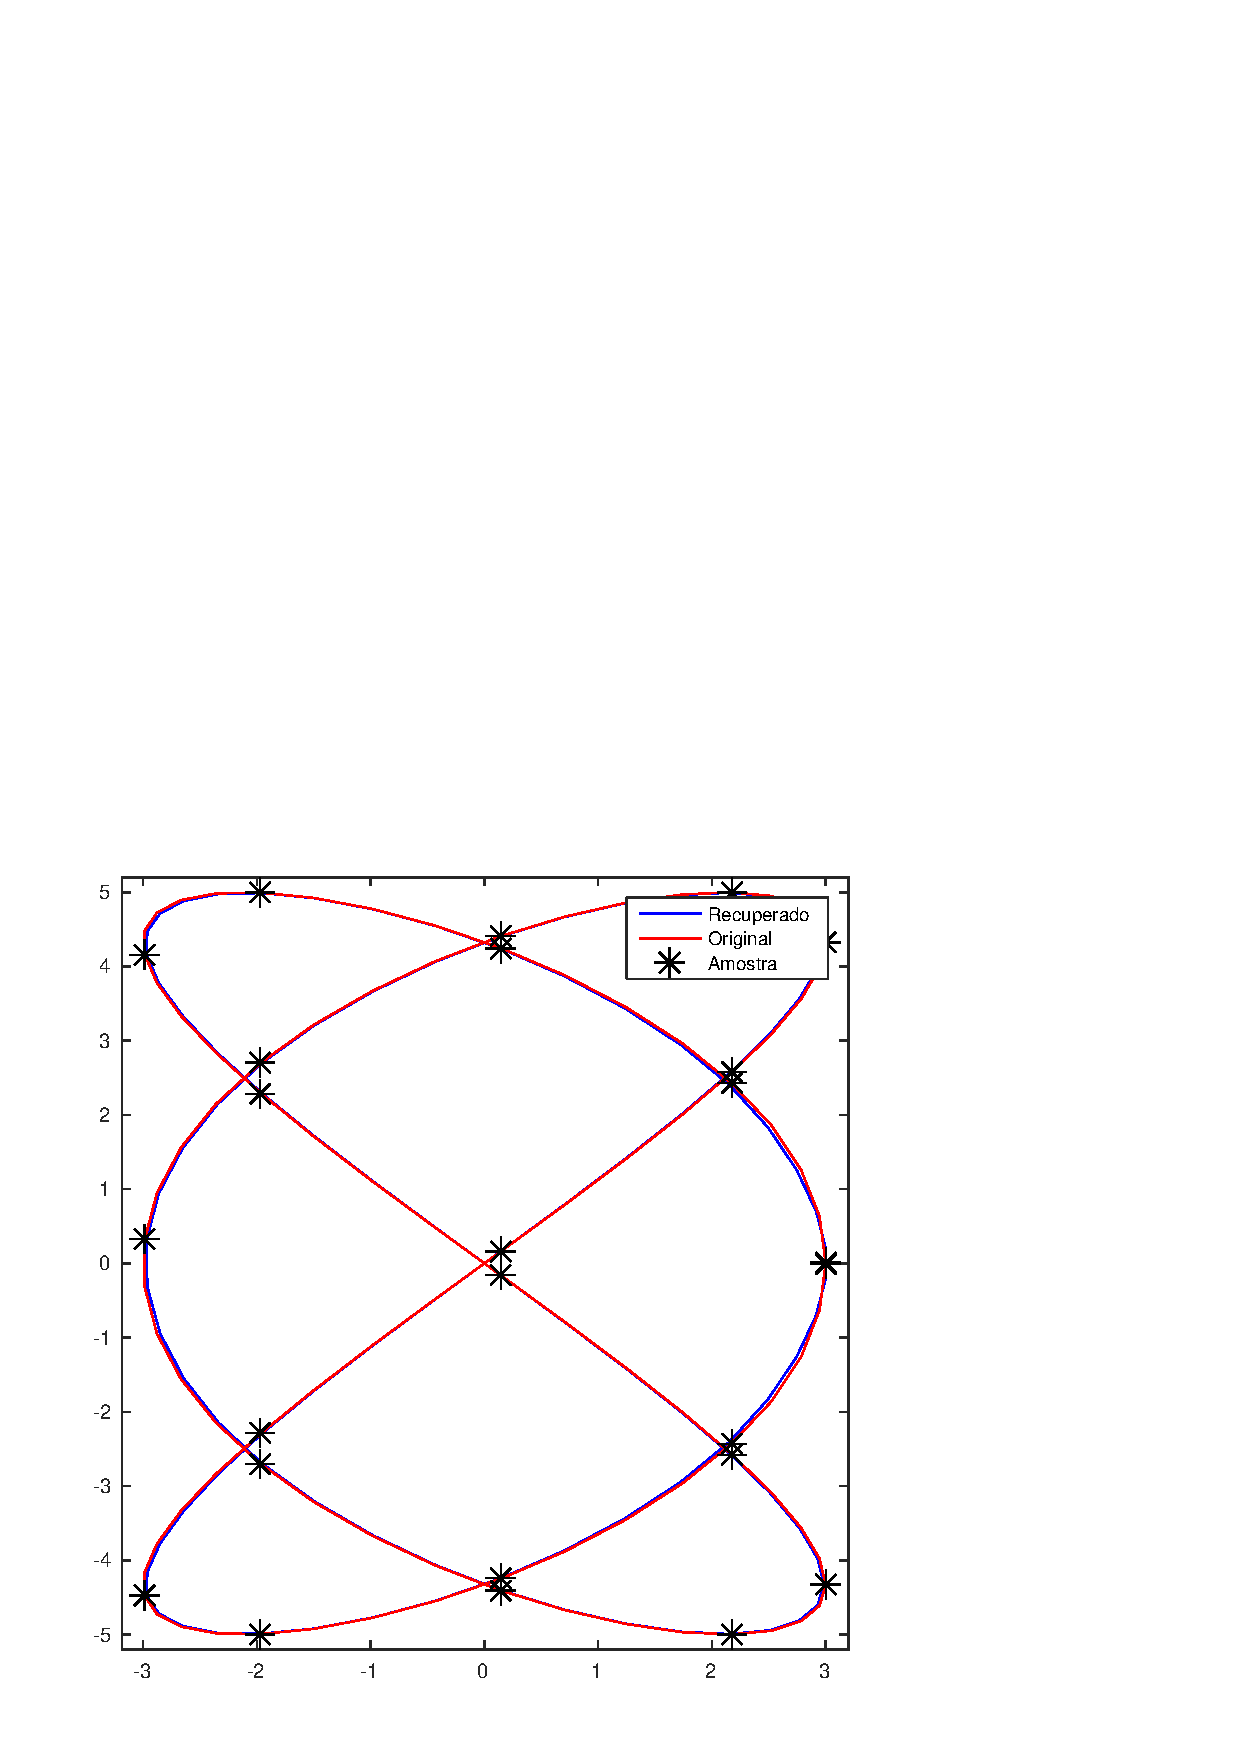
\includegraphics[trim={5cm 2cm 3cm 2cm},clip,width=\textwidth]{img/rep_2_25.jpg}
		\caption{25 pontos. Erro = 2.0368}
		\label{fig:ex23}
	\end{subfigure} %[3 * cos(3 * t); 5 * sin(2 * t)]';
	\legend{Fonte: Elaborada pelo autor.}
	\label{fig:ex2rep}
\end{figure}

Como dito anteriormente, neste projeto, os pontos âncora escolhidos serão as características robustas da curva. Embora isto ainda não tenha sido implementado, pode-se ver na figura \ref{fig:repcurv} a reconstrução da curva a partir da escolha de pontos de maior curvatura, calculada como mostrada na seção \ref{sec:curvdisc}. Os pontos escolhidos estão destacados em azul, a curva original está representada em vermelho e a curva reconstruída, em azul.

\begin{figure}[ht!]
	\centering
	\caption{Representação da curva do contorno da folha, utilizando pontos de maior curvatura como amostra.}
	\begin{subfigure}[t]{0.31\textwidth}
		\centering
		\includegraphics[width=\textwidth]{img/curv45.jpg}
		\caption{45 pontos. Erro $11971.34$}
		\label{fig:ex31}
	\end{subfigure}
	\hfill
	\begin{subfigure}[t]{0.31\textwidth}
		\centering
		\includegraphics[width=\textwidth]{img/curv70.jpg}
		\caption{70 pontos. Erro $762.87$}
		\label{fig:ex32}
	\end{subfigure}
	\hfill
	\begin{subfigure}[t]{0.31\textwidth}
		\centering
		\includegraphics[width=\textwidth]{img/curv100.jpg}
		\caption{100 pontos. Erro $712.67$}
		\label{fig:ex33}
	\end{subfigure}
	\legend{Fonte: Elaborada pelo autor.}
	\label{fig:repcurv}
\end{figure}

O contorno original da folha possui $1472$ pontos, no intervalo $x \in [46, 299]$, $y \in [68, 761]$. Por mais que a escolha dos pontos âncora não tenha sido feita de forma adequada (e será melhorada na próxima etapa do projeto), os erros apresentados foram baixos, considerando a curva em análise.

A escolha dos $m$ pontos âncora foi realizada da seguinte forma: todos os pontos da curva foram ordenados de forma decrescente com relação ao valor da curvatura. Após isso, todos os $n$ pontos foram divididos em $K$ grupos linearmente espaçados (cada um com $\lfloor n/k \rfloor$ pontos, e os $n \mod k$ primeiros grupos com um ponto a mais), e foram escolhidos os primeiros $\lfloor m/k \rfloor$ pontos de cada grupo (e um ponto a mais dos primeiros $m \mod k$ grupos). Isto foi feito para aumentar a representatividade de pontos âncoras ao longo da curva, e não escolher apenas aqueles concentrados em região de maior curvatura que, no caso da folha, estão concentrados na porção inferior do contorno.

Esta escolha foi feita para teste, e será melhorada para a próxima etapa, com a escolha dos pontos importantes como pontos âncora.